\section{Introduction}
    
    The mitral valve (MV) is the most structurally complex and physically demanded valve within the heart. It is one of the most suitable choices for the development and validation of a generalized meso-scale structural constitutive model (MSSCM). According the American Heart Association in 2013, it is estimated that MV disease is present in over 4 million adults \cite{go_heart_2014}. MV regurgitation is the most common pathology resulting from myocardial infarction (ischemic mitral regurgitation or IMR). The most frequent corrective approach used to restore leaflet function is MV annuloplasty \cite{kaneko_mitral_2014, amini_vivo_2012}, wherein an annuloplasty ring is used to induce MV leaflet closure during systole. However, such procedures alter the distribution of stress within the leaflet \cite{amini_vivo_2012,salgo_effect_2002,mahmood_three_2009,jimenez_saddle_2007,padala_saddle_2009,sacks_vivo_2006,eckert_vivo_2009,rausch_vivo_2011}, which may influence the long-term durability of the repair procedure. Long-term studies suggests that 60\% of patients who underwent MV repair show recurrence of MV regurgitation within 3–5 years, and 10–15\% of patients require re-operation within the following 10 years \cite{flameng_recurrence_2003,flameng_durability_2008}. The need for computational models, based on understanding of the underlying mechanobiological processes is self-evident for predicting the outcome of surgically repaired MVs and driving the development of improved patient-specific surgical techniques.
    
    
    While MV leaflets may first appear essentially to be membranous flaps, they are in actuality complex multilayered structures that undergo large anisotropic deformations in vivo \cite{sacks_vivo_2006}. Specifically, there are four morphologically distinct layers of the MV: the ventricularis, fibrosa, spongiosa, and atrialis \cite{carruthers_alterations_2012}. All layers are composed of various amounts of dense networks of collagen (mostly type I) and elastin fibers, as well as non-fibrous proteoglycans (PG) and glycosaminoglycans (GAG). In a recent study \cite{lee_quantification_2015}, we demonstrated that the layer-specific deformations of the MV interstitial cells (MVIC) are a direct result of the layer-specific architectures. This suggests that layer-specific adaptations are possible, as observed in Wells et al.\cite{wells_physiological_2012}. Yet, it remains unclear as to (1) why the MV has this distinct pattern of layers, (2) what the respective mechanical roles of each layer are, and (3) how does these patterns relate to the bulk macro-scale responses.
    
    
    The underlying layer-specific differences in mechanical properties are a result from the constituent fiber populations. Type I collagen is the most abundant protein found in MV tissue, and it is the major determinant of its mechanical behavior \cite{parry_molecular_1988,gelse_collagens_2003}. The functional subunit of collagen is the collagen fibril, which composed of tropocollagen molecules that arrange themselves into a quarter stacking array \cite{parry_molecular_1988,gelse_collagens_2003}. It is this structure that allows small angle X-ray scattering (SAXS) studies to measure the underlying fibril deformations for tendon \cite{sasaki_elongation_1996,sasaki_stress_1996} and MV leaflet tissues \cite{liao_relation_2007}. At the next structural level, the collagen fibrils group to form collagen fibers. There is an incomplete understanding regarding the functional relationship between collagen fibers and the fibrils. In fact, the exact definition of collagen fibers in relation to fibrils is usually tissue specific. Like the fibrils from which their functional properties are derived, collagen fibers exhibit tensile strength of up to 1 GPa \cite{shen_stress_2008,gentleman_mechanical_2003,eppell_nano_2006,yang_mechanical_2008,sacks_biomechanics_2009} with low flexural stiffness \cite{sacks_biomechanics_2009}. As a result, collagen fibers typically extend by no more than a 4–5\%. To increase the tissue-level compliance, collagen fibers at the macroscopic scale become sinusoidally crimped \cite{parry_molecular_1988} and does not contribute mechanically until fully straightened. Moreover, the distribution of collagen fiber-level straightening strains is the mechanism for tissue-level non-linearity \cite{lanir_constitutive_1983,sacks_multiaxial_2003}. 
    
    
    In contrast to collagen, elastin forms complex cross-linked fibrous networks with comparatively low modulus that are thought to assist in tissue recoil \cite{debelle_elastin_1999,debelle_structures_1999} and maintaining collagen fiber crimp \cite{vesely_comparison_1998,scott_aortic_1995}. Unlike large arteries, elastin is present in much lower quantities in valvular tissues compared to collagen \cite{sacks_biomechanics_2009,vesely_comparison_1998,lis_biochemical_1987,stella_biaxial_2007} and its role in valve mechanics is not well understood. Finally, we note that glycosaminoglycans (GAGs) are known to affect water retention and hysteresis in valvular tissues \cite{lovekamp_stability_2006,eckert_biomechanical_2013}, with the loss of GAGs known to reduce cuspal thickness and diminish rehydration capacity. However, GAGs are not a primary load bearing component, but appear act as a dampening mechanism to smooth rapid bending motions of the leaflet during valve function \cite{eckert_biomechanical_2013}.
    
    
    Thus, a more complete understanding of MV function and failure must involve an improved understanding of how the above MV leaflet structures mechanically interact. This is best done through the mathematical development of constitutive models that incorporate these features, which can aid both in providing insight and in forming a predictive modeling framework for their remodeling and failure. In the present, work we developed a novel comprehensive meso-scale (i.e. at the level of the fiber) structural constitutive model (MSSCM) for MV leaflets, focusing on the specific collagen and elastin fiber networks within each of its four distinct layers. We used a comprehensive set of structural and mechanical studies (Table \ref{c2tab:experiments}) and a rigorous experimentally guided approach to tackle model formulation, parameter optimization and model validation (Fig. \ref{c2:fig:1}). The results were then validated at both the micro (fibril) and tissue-level using a novel approach based on a previous SAXS study on the mitral valve \cite{liao_relation_2007}, and again at the meso-scale using measured fiber structures. We also explored a novel extension to previous structural constitutive model approaches \cite{hollander_constitutive_2011,chen_micromechanics_2011,fata_insights_2014,sacks_incorporation_2003} to allow for angular dependency of collagen fiber recruitment (orientation-variant) and assessed the model predictive capabilities under extra physiological loading that could occur in post-surgical scenarios.
    
\begin{table}
\centering
\caption{Experimental Techniques and Deliverables}\label{c2tab:experiments}
 \begin{tabular}{|m{.15in}|L{0.6in}|L{1in}|L{2.4in}|L{0.95in}|}
 \hline
 &  \textbf{Study}  & \textbf{Description}  & \textbf{Purpose}  & \textbf{Description}  \\
 \hline
 
 \multirow{7}{*}{\rotatebox[origin=c]{90}{Structure}}
 & SHG  
 & Image of fluorescently labeled collagen and elastin 
 & Image processing is done to quantify the fiber orientation distribution function of collagen and elastin within each layer. 
 & ODF (used for validation) \\
 \cline{2-5}
 
 & Histology
 & Collagen, elastin and Proteoglycans are stained in a transmural slice. 
 & The image is separated into channels and is used to quantify the mass fractions and relative fraction of collagen and elastin of each layer. This is used directly in the model. 
 & Mass fractions   \\
 \hline
 
 \multirow{22}{*}{\rotatebox[origin=c]{90}{Mechanical}}
 & SAXS
 & X-ray scattering at a length comparable to D-period of the fiber
 & The SAXS scatter pattern have periods related to the D-period of the collagen fibers. The D-period can be used to quantify the fiber-level strain and the fiber stiffness
 & Collagen Fiber Modulus, (for validation)   \\
 \cline{2-5}
 
 & Planar Biax (EB)
 & Biax with equal strain along both axes
 & Under equibiaxial strain, we can recover the ensemble stress from the sum of the axial stresses. This allows us to model the ensemble stress directly to determine the fiber modulus and fiber recruitment.
 & \multirow{8}{0.95in}{Collagen Fiber Modulus, Recruitment Parameters (For validation)}  \\
 \cline{2-4}
 
 & Uniaxial	
 & Tissue is deformed along the preferred direction of the fibers
 & With the tight splay, under uniaxial extension all fibers become nearly aligned to the test axis, allowing us to use a simplified model rather like using the ensemble stress to recover the fiber modulus and recruitment. 	& \\
 \cline{2-5}
 
 & Planar Biax (Multi-prot)	
 & Data is taken over the physiological and extra-physiological range.	
 & This with us the data to performed parameter estimation to determine the properties of the MV. The outer extra-physiological protocols can be used check the predictive ability of the model. 
 & Layer dependent material properties.     \\
 \hline
 
 \end{tabular}
\end{table}





%%%%%%%%%%%%%%%%%%%%	begin FIGURE 	%%%%%%%%%%%%%%%%%%%%
\begin{figure}
\centering
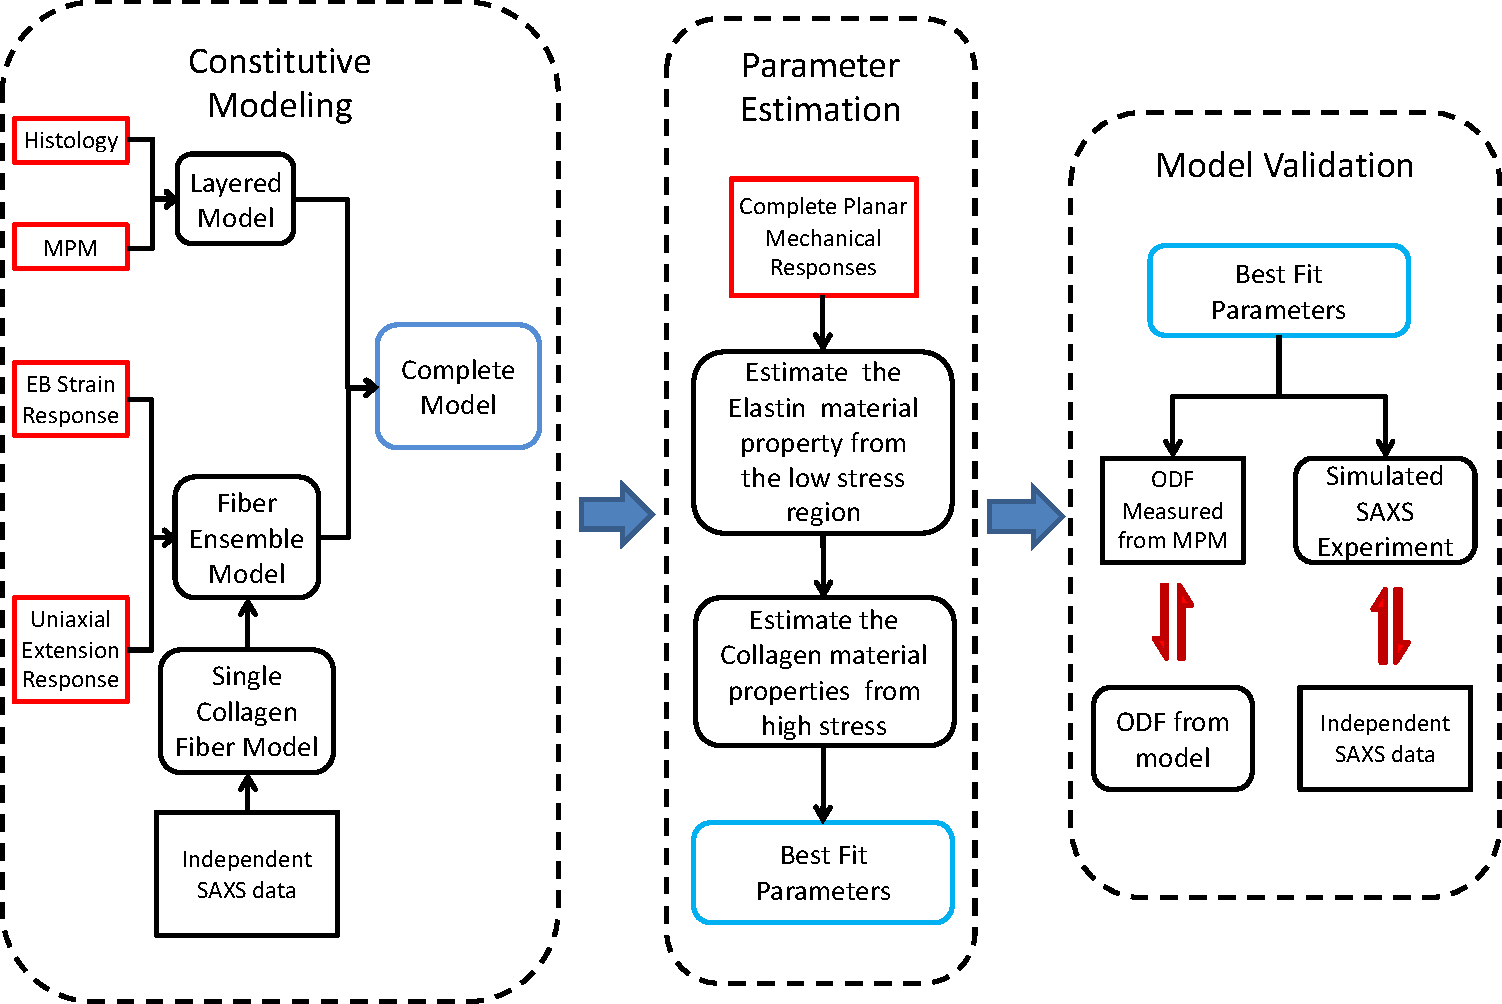
\includegraphics[width=\textwidth]{Images/chapter2/figure1.pdf}
\caption{Our modeling approach can be divided into 3 parts: (1) constitutive modeling, where we use both structural and mechanical data to guide model formulation. (2) Parameter estimation, where we used a detailed sequential approach to narrow down the optimal parameters. (3) Model validation, where we used SAXS and MPM to validate the model at both the micro- and meso-scale.}
\label{c2:fig:1}
\end{figure}
%%%%%%%%%%%%%%%%%%%%	 end FIGURE 	%%%%%%%%%%%%%%%%%%%%






